\documentclass[12pt,letterpaper]{article}
\usepackage{graphicx,textcomp}
\usepackage{subcaption}
\usepackage{natbib}
\usepackage{setspace}
\usepackage{fullpage}
\usepackage{color}
\usepackage[reqno]{amsmath}
\usepackage{amsthm}
\usepackage{fancyvrb}
\usepackage{amssymb,enumerate}
\usepackage[all]{xy}
\usepackage{endnotes}
\usepackage{lscape}
\newtheorem{com}{Comment}
\usepackage{float}
\usepackage{hyperref}
\newtheorem{lem} {Lemma}
\newtheorem{prop}{Proposition}
\newtheorem{thm}{Theorem}
\newtheorem{defn}{Definition}
\newtheorem{cor}{Corollary}
\newtheorem{obs}{Observation}
\usepackage[compact]{titlesec}
\usepackage{dcolumn}
\usepackage{tikz}
\usetikzlibrary{arrows}
\usepackage{multirow}
\usepackage{xcolor}
\newcolumntype{.}{D{.}{.}{-1}}
\newcolumntype{d}[1]{D{.}{.}{#1}}
\definecolor{light-gray}{gray}{0.65}
\usepackage{url}
\usepackage{listings}
\usepackage{color}

\definecolor{codegreen}{rgb}{0,0.6,0}
\definecolor{codegray}{rgb}{0.5,0.5,0.5}
\definecolor{codepurple}{rgb}{0.58,0,0.82}
\definecolor{backcolour}{rgb}{0.95,0.95,0.92}

\lstdefinestyle{mystyle}{
	backgroundcolor=\color{backcolour},   
	commentstyle=\color{codegreen},
	keywordstyle=\color{magenta},
	numberstyle=\tiny\color{codegray},
	stringstyle=\color{codepurple},
	basicstyle=\footnotesize,
	breakatwhitespace=false,         
	breaklines=true,                 
	captionpos=b,                    
	keepspaces=true,                 
	numbers=left,                    
	numbersep=5pt,                  
	showspaces=false,                
	showstringspaces=false,
	showtabs=false,                  
	tabsize=2
}
\lstset{style=mystyle}
\newcommand{\Sref}[1]{Section~\ref{#1}}
\newtheorem{hyp}{Hypothesis}

\title{Problem Set 1}
\date{Due: October 1, 2023}
\author{Applied Stats/Quant Methods 1}

\begin{document}
	\maketitle
	
	\section*{Instructions}
	\begin{itemize}
	\item Please show your work! You may lose points by simply writing in the answer. If the problem requires you to execute commands in \texttt{R}, please include the code you used to get your answers. Please also include the \texttt{.R} file that contains your code. If you are not sure if work needs to be shown for a particular problem, please ask.
\item Your homework should be submitted electronically on GitHub.
\item This problem set is due before 23:59 on Sunday October 1, 2023. No late assignments will be accepted.
\item Total available points for this homework is 80.
	\end{itemize}
	
	\vspace{1cm}
	\section*{Question 1 (40 points): Education}

A school counselor was curious about the average of IQ of the students in her school and took a random sample of 25 students' IQ scores. The following is the data set:\\
\vspace{.5cm}

\lstinputlisting[language=R, firstline=36, lastline=36]{/Users/poisson/Documents/GitHub/Fork_Statsl Fall2023/problemSets/PS01/template/PS01.R}  

\vspace{1cm}

\begin{enumerate}
	\item Find a 90\% confidence interval for the average student IQ in the school.\\
\newpage
		 \textbf{Input}\\
			\lstinputlisting[language=R, firstline=58, lastline=80]{PS01_answersFL.R} 
		
		  \textbf{Output}\\\\
		   \noindent The 90\% confidence interval for the average student IQ in the school is: 93.96~102.92 
		
		
	\item Next, the school counselor was curious  whether the average student IQ in her school is higher than the average IQ score (100) among all the schools in the country.\\ 
	
	\noindent Using the same sample, conduct the appropriate hypothesis test with $\alpha=0.05$.\\
	
	\textbf{Research Hypothesis}
		\begin{itemize} 
\item Null Hypothesis: The average student IQ in the school is the same as the average IQ score among all the schools in the country → $\mu = 100$
\item Alternative Hypothesis: The average student IQ in the school is higher than the average IQ score among all the schools in the country → $\mu > 100$
		\end{itemize}
		
\newpage
		
		\noindent \textbf{Input}\\
				\lstinputlisting[language=R, firstline=92, lastline=93]{PS01_answersFL.R} 
				
		\noindent \textbf{Output}
		\begin{verbatim}
				One Sample t-test
				data:  y 
				t = -0.59574, df = 24, p-value = 0.7215
				alternative hypothesis: true mean is greater than 100
				95 percent confidence interval: 93.95993      Inf
				sample estimates:
				mean of x     
				98.44 
		\end{verbatim}
		
		\textbf{Conclusion}\\\\
		\noindent $p = 0.7215 > \alpha=0.05$ \\\\Therefore, the evidence cannot reject null hypothesis and accept alternative hypothesis. We are unable to conclude that the average student IQ in the school is higher than the average IQ score among all the schools in the country.
\end{enumerate}

\newpage

	\section*{Question 2 (40 points): Political Economy}

\noindent Researchers are curious about what affects the amount of money communities spend on addressing homelessness. The following variables constitute our data set about social welfare expenditures in the USA. \\

\begin{tabular}{r|l}
	\texttt{State} &\emph{50 states in US} \\
	\texttt{Y} & \emph{per capita expenditure on shelters/housing assistance in state}\\
	\texttt{X1} &\emph{per capita personal income in state} \\
	\texttt{X2} &  \emph{Number of residents per 100,000 that are "financially insecure" in state}\\
	\texttt{X3} &  \emph{Number of people per thousand residing in urban areas in state} \\
	\texttt{Region} &  \emph{1=Northeast, 2= North Central, 3= South, 4=West} \\
\end{tabular}

\vspace{.5cm}
\noindent Explore the \texttt{expenditure} data set and import data into \texttt{R}.
\vspace{.5cm}
\lstinputlisting[language=R, firstline=54, lastline=54]{/Users/poisson/Documents/GitHub/Fork_Statsl Fall2023/problemSets/PS01/template/PS01.R}  

\begin{itemize}

\item
Please plot the relationships among \emph{Y}, \emph{X1}, \emph{X2}, and \emph{X3}? What are the correlations among them (you just need to describe the graph and the relationships among them)?


\begin{figure}[h!]
	\centering
	\begin{subfigure}[b]{0.45\textwidth}
		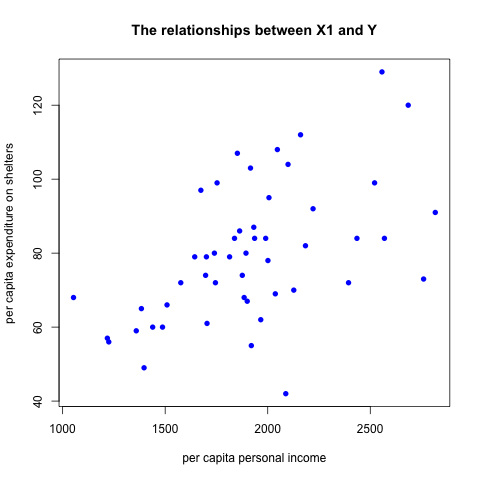
\includegraphics[width=\textwidth]{PS01_Q2_scplot1.png}
		\label{fig:image1}
	\end{subfigure}
	\hspace{.5cm} 
	\begin{subfigure}[b]{0.45\textwidth}
		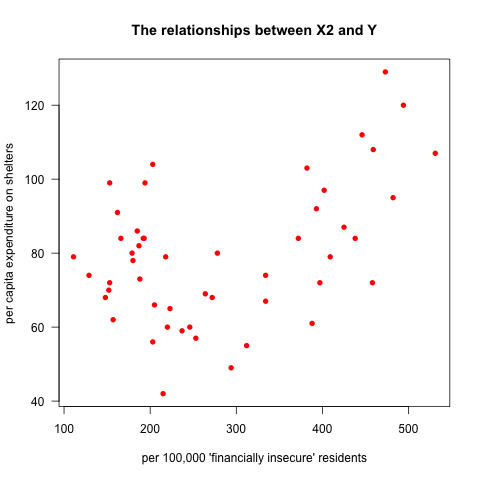
\includegraphics[width=\textwidth]{PS01_Q2_scplot2.png}
		\label{fig:image2}
	\end{subfigure}
	\label{fig:main}
\end{figure}

\emph{X1 and Y :} From the graph, it can be observed that there is a positive correlation between per capita personal income and per capita expenditure on shelters: as per capita personal income increases, per capita expenditure on shelters also increases. Most of the data points are distributed within the range of 1600 to 2200 on the x-axis and 60 to 110 on the y-axis. \\
\emph{X2 and Y :} There is no obvious linear correlation between 'per 100,000 financially insecure residents' and 'per capita expenditure on shelters'. However, the data shows a downward trend followed by an upward trend, with a turning point around 300 on the x-axis. There might be a nonlinear correlation that needs further investigation.

\begin{figure}[h!]
	\centering
	\begin{subfigure}[b]{0.45\textwidth}
		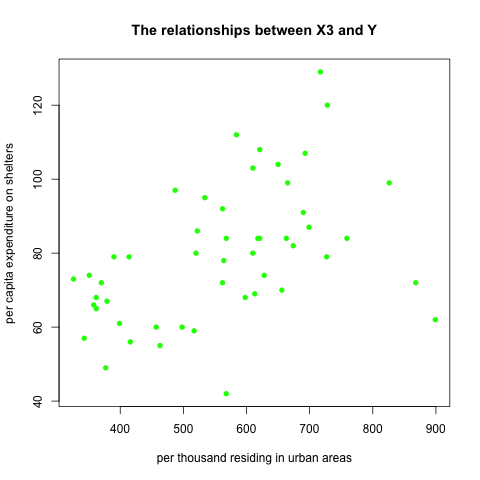
\includegraphics[width=\textwidth]{PS01_Q2_scplot3.png}
		\label{fig:image1}
	\end{subfigure}
	\hspace{.5cm} 
	\begin{subfigure}[b]{0.45\textwidth}
		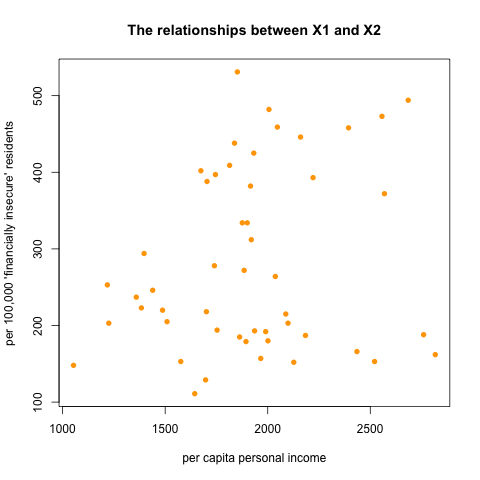
\includegraphics[width=\textwidth]{PS01_Q2_scplot4.png}
		\label{fig:image2}
	\end{subfigure}
	\label{fig:main}
\end{figure}

\emph{X3 and Y :} There is a positive correlation between "per thousand residing in urban areas" and "per capita expenditure on shelters". Most of the data points are distributed in the range of 350 to 700 on the x-axis and 60 to 110 on the y-axis. One outlier is located around 570 on the x-axis, and the other two around 900 on the x-axis.\\
\emph{X1 and X2 :} There is no correlation between per capita personal income and per 100,000 financially insecure residents.


\begin{figure}[h!]
	\centering
	\begin{subfigure}[b]{0.45\textwidth}
		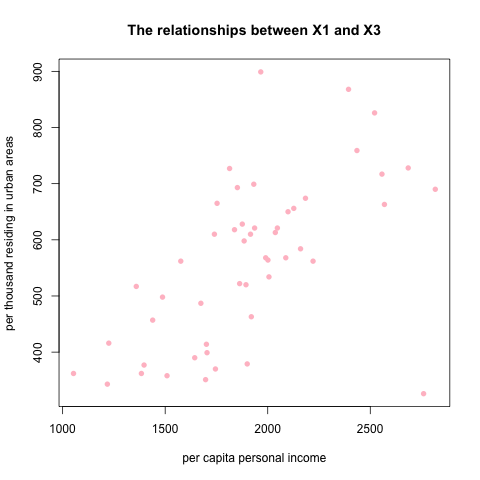
\includegraphics[width=\textwidth]{PS01_Q2_scplot5.png}
		\label{fig:image1}
	\end{subfigure}
	\hspace{.5cm} 
	\begin{subfigure}[b]{0.45\textwidth}
		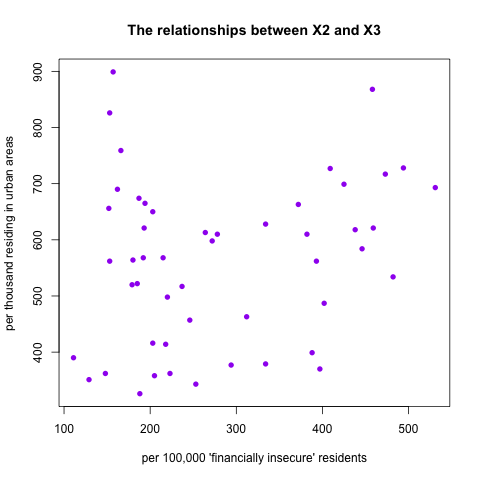
\includegraphics[width=\textwidth]{PS01_Q2_scplot6.png}
		\label{fig:image2}
	\end{subfigure}
	\label{fig:main}
\end{figure}

\newpage

\emph{X1 and X3 :} There is a positive correlation between per capita personal income and per thousand residing in urban areas. The majority of data points are distributed in the range of 1500 to 2200 on the horizontal axis and 350 to 700 on the vertical axis. There are two outliers, one at 2000 on the horizontal axis and 900 on the vertical axis, and another at 2700 on the horizontal axis and 310 on the vertical axis. These outliers might require further  handling.\\
\emph{X2 and X3 :} There is no correlation between per thousand residing in urban areas and per 100,000 financially insecure residents.

\vspace{1.5cm}


\item
Please plot the relationship between \emph{Y} and \emph{Region}? On average, which region has the highest per capita expenditure on housing assistance?

	\begin{figure}[h!]\centering
	\label{fig:plot_1}
	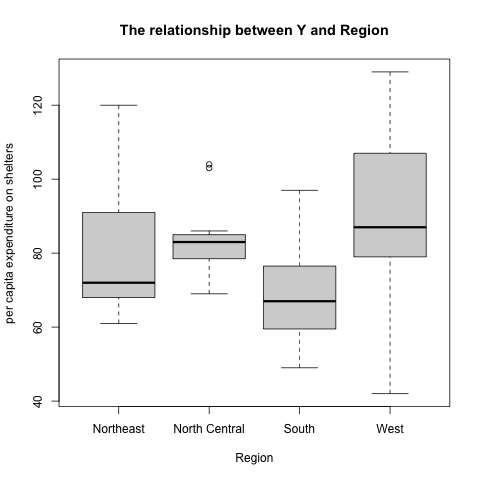
\includegraphics[width=.70\textwidth]{PS01_Q2_scplot8.png}
   \end{figure}
   
   From this boxplot, the region of \emph{West} has the highest per capita expenditure on housing assistance.

\newpage

\item
Please plot the relationship between \emph{Y} and \emph{X1}? Describe this graph and the relationship. Reproduce the above graph including one more variable \emph{Region} and display different regions with different types of symbols and colors.

	\begin{figure}[h!]\centering
	\label{fig:plot_1}
	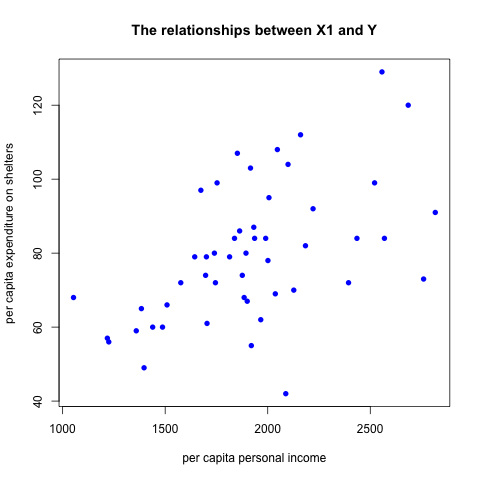
\includegraphics[width=.50\textwidth]{PS01_Q2_scplot1.png}
\end{figure}

\emph{X1 and Y :} In general, the correlation between per capita personal income and per capita expenditure on shelters is positive. However, after the income surpasses 2000, with the increase in x, the central tendency begins to weaken and the data becomes more discrete. 

\begin{figure}[h!]\centering
	\label{fig:plot_1}
	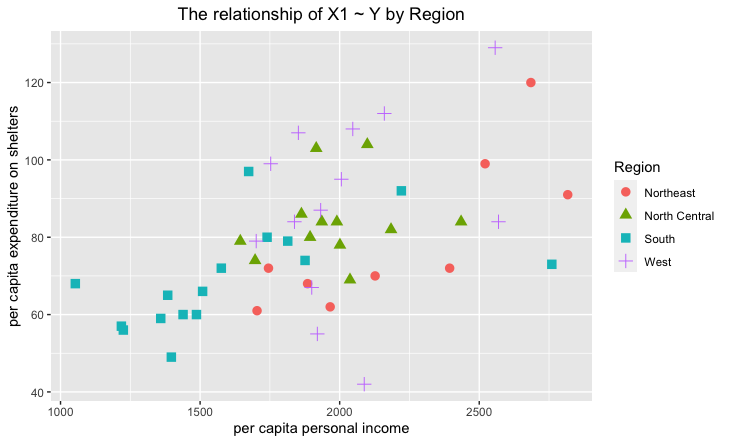
\includegraphics[width=.85\textwidth]{PS01_Q2_scplot9.png}
\end{figure}

\end{itemize}

\end{document}
